% !TEX root = ../thesis_main.tex



\clearpage	
\chapter{Results}
\label{results_chapter}
\note[color=jb]{JB:  Dan and I independently discussed Ch 10 yesterday, and he has suggestions to
help. So I will also schedule a meeting with Dan and you to discuss
Ch 10 Results and whether the S,T part must be deleted and left to a paper.
You don't have enough time, and although this should be quite straightforward,
it is not your critical result and it's the only thing that can go.}

\section{Measured Limits on $b_{Fierz}$, $C_S$, $C_T$}
	%\\*
	Results go here, with measured limits described and quantified in all formats anyone could ever care about.
	
\begin{figure}[h!!!t]
	\centering
	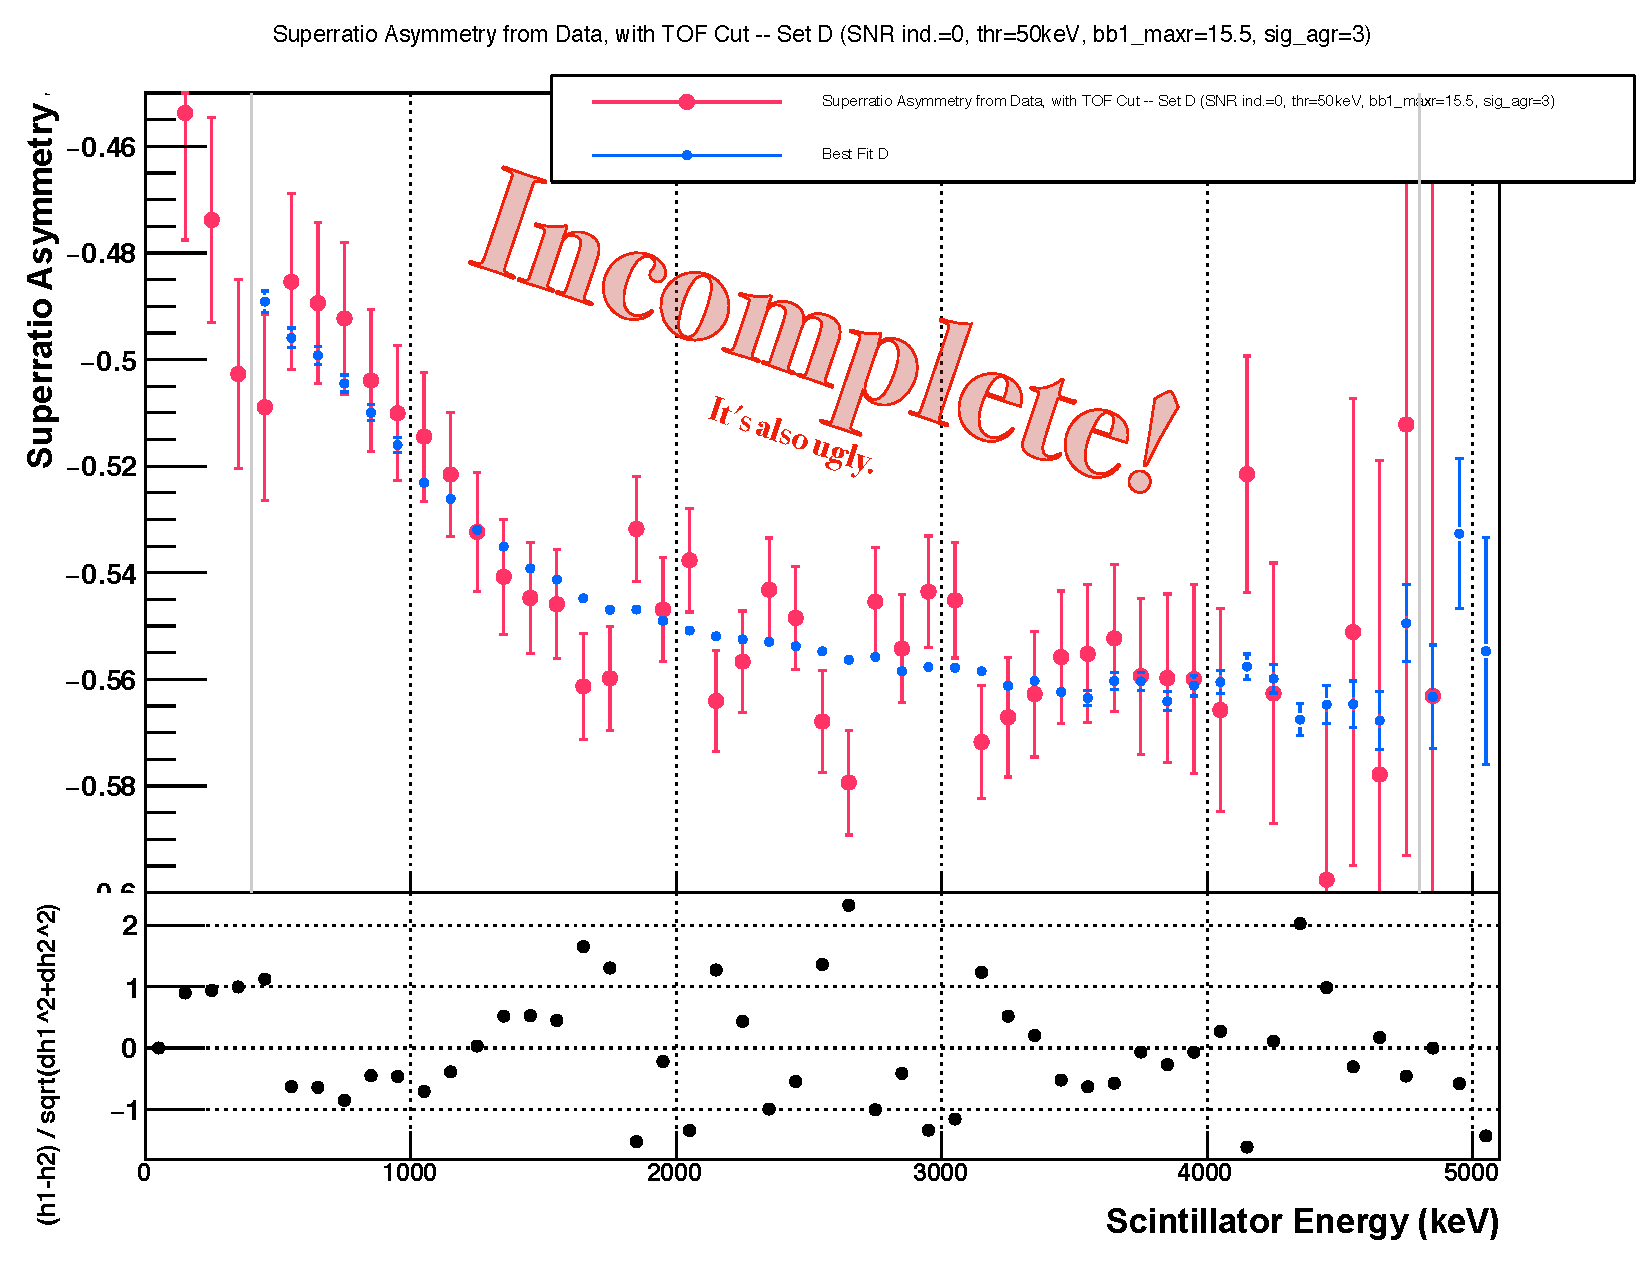
\includegraphics[width=.999\linewidth]
	{Figures/AsymmetryAndResiduals.pdf}
	\caption{A superratio asymmetry from the data, and the best fit from simulations.}	
	\label{fig:asymmetry}
\end{figure}
	
	
\begin{figure}[h!!!t]
	\centering
	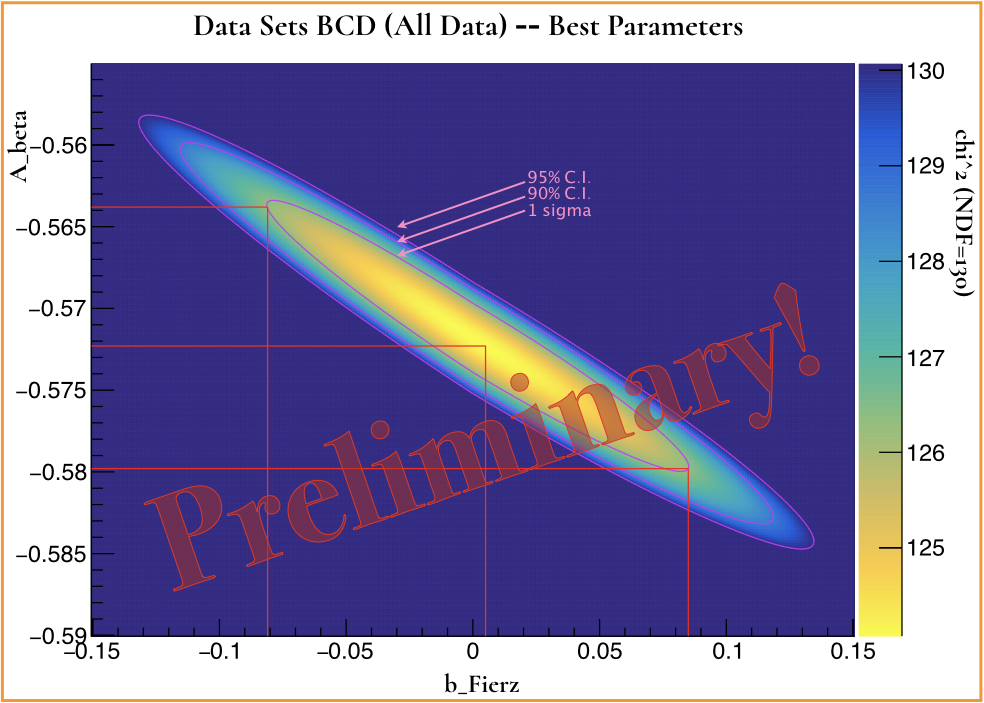
\includegraphics[width=.999\linewidth]
	{Figures/Abeta_bFierz_2D_prelim.png}
	\caption{Some results.  I'll want to show at least one of these things.  Probably show a separate one for each runset, actually.}	
	\label{fig:2d_results_bcd}
\end{figure}

\section{Discussion of Corrections and Uncertainties}
	...
	
\section{Relation to Other Measurements and New Overall Limits}
	%\\*
	In which I'll show exclusion plots and write down new limits, combining my result with results from the literature.
	Or, y'know, maybe I'll just talk about doing that.
	
\note[color=jb]{JB says:   To put your work in context, please add at the end of that minimal S,T section, or at the end of "Our Decay" section
\\ ... \\
The best existing measurement of $\bFierz$ is in the decay of the neutron~\cite{Saul2020},
$\bFierz$ = 0.017 $\pm$ 0.021, consistent with the Standard Model prediction of zero.
Our measurement is strongly related, yet complementary.
In terms on non-Standard Model Lorentz current structures, to lowest order in the non-SM  currents the same equation applies:
\\
$\bFierz$ = $\pm$ $(C_S +C_S' + (C_T - C_T') \lambda^2)/( 1 + \lambda^2)$
\\
(the plus is for $\beta^-$ decay and the - for $\beta^+$ decay)~\cite{jtw}.  [to be continued...] }

\note[color=jb]{[...continued from prev.]
\\
In our $^{37}$K case, $\lambda^2$ = $|M_{\rm GT}|^2$/$|M_{\rm F}|^2$ is close to 3/5 (the expected value j/(j+1) for a single j=3/2 d3/2 nucleon)~\cite{deShalit1963},
while for the neutron $\lambda^2$ is close to 3 (the expected value for an (j+1)/j j=1/2 s1/2 nucleon).
$|M_F|$, the Fermi matrix element, is nearly the same for both of these isospin = 1/2 decays (the largest correction is the larger isospin mixing of $\sim$0.01 in $^{37}$K).
So our observable is relatively less sensitive to Lorentz tensor currents, and will predominantly constrain or discover Lorentz scalar currents.
\\...\\ 
Full considerations would require a weighted fit of $\bFierz$ experiments and similar observables~\cite{Falkowski2021}, and are beyond the scope of this thesis.
The info from this thesis, values of $\Abeta$ and $\bFierz$ with their uncertainties, can together with the known $fT$ value (lifetime and
branching ratio) allow the community and/or the collaboration to include the results in a future constraint or discovery of scalar and tensor Lorentz currents
contributing to $\beta$ decay.}


\section{Conclusions and Future Work}
